\section{Auswertung}
\label{sec:Auswertung}
\subsection{Aufnahme eines Emissionspektrums der Kupfer Röntgenröhre}
\paragraph{}
Das Röntgenspektrum der Kupfer Röntgenröhre \cite{AL} werden in 0,1°-Schritten in Bereich  von \(8° \leq \alpha \leq 25°\) und in \autoref{fig:EmissionCu} veranschaulicht.

\begin{figure}
  \centering
  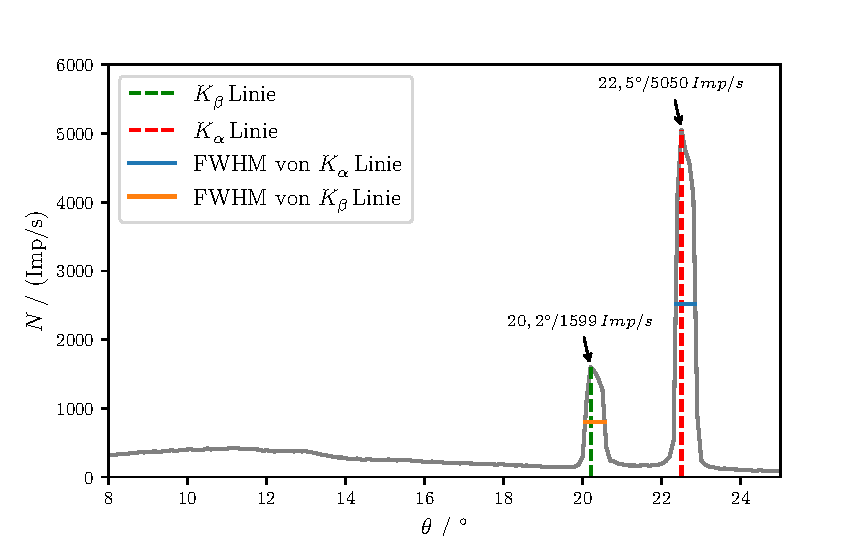
\includegraphics{EmissionCu.pdf}
  \caption{EmissionCu.}
  \label{fig:EmissionCu}
\end{figure}
 
Aus der \autoref{fig:EmissionCu} werden Intensitäten und Kristallwinkeln bei dem ersten und zweiten Bergen (entsprechen für $K_\alpha$- und $K_\beta$-Linie von Kupfer Emissionspektrum) notiert.

Für $K_\beta$-Linie: \(\theta=20,2°\); \(N=1599 \,\mathrm{Imp/s}\).

Für $K_\alpha$-Linie: \(\theta=22,5°\); \(N=5050 \, \mathrm{Imp/s}\). 

\paragraph{}
Die entsprechende Energien werden durch die Formel
\begin{equation}
  E = \frac{hc}{\lambda}\\
 \end{equation}
mit den durch die Formel (3) gerechneten Wellenlängen $\lambda$
bestimmt und ergeben sich zu
\begin{align*}\mathrm{keV}
  E_\alpha &= 8,059\,\mathrm{keV}\\
  E_\beta &= 8,931 \,\mathrm{keV}.\\
\end{align*}


\subsection{ Bestimmung der Transmission als Funktion der Wellenlänge}
\paragraph{}
Die Zählrate der Röntgenstrahlung mit Aluminium-Absorber $N_{Al}$ und ohne Aluminium-Absorber $N_0$ im Schritten von \( \Delta \alpha= 0,1° \) werden notiert.\cite{AL} (Messzeit \(\Delta t=200 \,s \))\\

Mit der Gleichung (4) werden die Zählrate $I_{Al}$ und $I_{0}$ mit der Totzeit \(\tau=90 \,\mu s \) bestimmt.

Die wahren Zählrate ist \(I^{*}=I \cdot \Delta t\).
\paragraph{}
Die Transmission \(T=\frac{{I^{*}}_{Al}}{{I^{*}}_{0}} =\frac{I_{Al}}{I_{0}}\) wird mit den gerechneten Werten von $I_{Al}$ und $I_{0}$ berechnet. 

Die entsprechenden Wellenlänge  $\lambda$ werden mit der Formel (3) ermittelt.
\paragraph{}
Die aus der Rechnungen erhaltenen Werte sind in Tabelle (1) aufgeführt.

Die Transmissionsfunktion $T(\lambda)$ in Abhängigkeit von $\lambda$ wird mit den Zählrate ($I_{Al}$) und ($I_{0}$) bestimmt:
\begin{equation}
  T(\lambda)=\frac{{I^{*}}_{Al}}{{I^{*}}_{0}} =\frac{I_{Al}}{I_{0}}={\frac{N_{Al}}{1-\tau N_{Al}}}\cdot {\frac{1-\tau N_{0}}{{ N_{0}}}}
\end{equation}
Die Ausgleichungsgerade hat die Form:
\begin{equation}
 y=a\cdot t+b 
\end{equation}
mit \(y=T(\lambda)\) und \(t= \lambda\).
Die Parameter ergeben sich zu
\begin{align*}
  a &=(-0,015195 \pm 0,000239)\,\mathrm{pm^{-1}}\\
  b &=(1,225073 \pm 0,014311).\\
 \end{align*}
 Die Fehler für Transmission $T$  wird dabei über die Gau"s´sche Fehlerfortfplanzung 
 \begin{equation}
     \Delta f = \sqrt{\sum_{i=1}^N {\Bigl(\frac{\partial f}{\partial y_i}\Bigr)^2 (\Delta y_i)^2}}
 \end{equation}

 \begin{align*}
  \Delta T =\sqrt{\Bigl(\frac{1}{I_{0}} \cdot \Delta {I}_{Al}\Bigr)^2+\Bigl(\frac{-{I}_{Al}}{{{I}_{0}}^2} \cdot \Delta {I}_{0}\Bigr)^2}
 \end{align*}
 berechnet.
Die Transmissionskurve und deren Ausgleichungsgerade sind in \autoref{fig:Transmissionskurve} graphisch stellen.


\begin{figure}
  \centering
  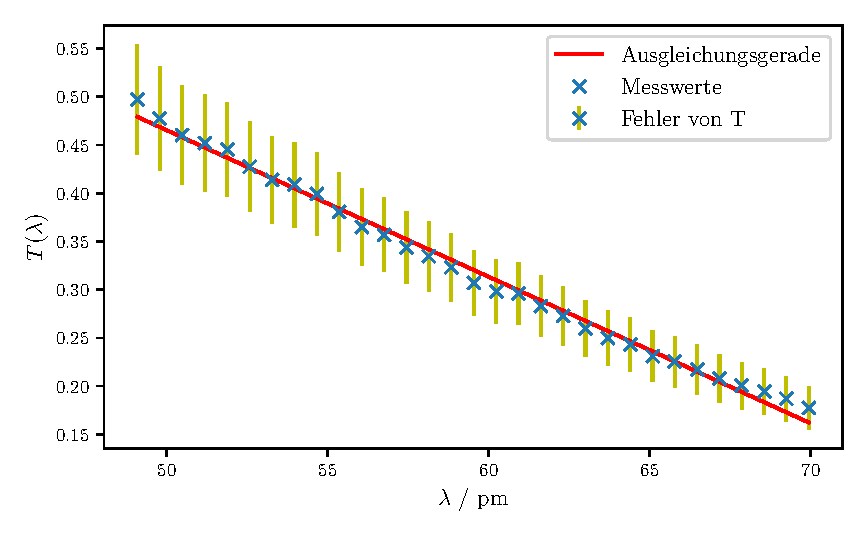
\includegraphics{Transmissionskurve.pdf}
  \caption{Transmissionskurve von Aluminium-Absorber.}
  \label{fig:Transmissionskurve}
\end{figure}


\begin{table}
  \centering
  \caption{Berechnete Daten für die Bestimmung der Transmission als Funktion der Wellenlänge.}
  \label{tab:some_data1}
  \begin{tabular}{ccccc}
    \toprule
    $\text{Kristallwinkeln} /\mathrm{°}$ & $I_{0} /\mathrm{Impulse}$  & $I_{Al} /\mathrm{ Impulse} $ & $T $ & $ \lambda  /\mathrm{pm}$\\
    \midrule 
7,0 & 230,692 & 114,671 & 0,497 & 49,089 \\
7,1 & 236,947 & 113,140 & 0,477 & 49,787 \\
7,2 & 245,821 & 113,140 & 0,460 & 50,484 \\
7,3 & 253,662 & 114,671 & 0,452 & 51,182 \\
7,4 & 260,990 & 116,203 & 0,445 & 51,879 \\
7,5 & 268,327 & 114,671 & 0,427 & 52,576 \\
7,6 & 275,674 & 114,161 & 0,414 & 53,273 \\
7,7 & 283,030 & 115,692 & 0,409 & 53,970 \\
7,8 & 288,291 & 115,182 & 0,400 & 54,666 \\
7,9 & 297,245 & 113,140 & 0,381 & 55,363 \\
8,0 & 303,046 & 110,590 & 0,365 & 56,059 \\
8,1 & 308,325 & 110,080 & 0,357 & 56,755 \\
8,2 & 317,310 & 109,060 & 0,344 & 57,451 \\
8,3 & 319,956 & 107,021 & 0,334 & 58,147 \\
8,4 & 326,310 & 105,492 & 0,323 & 58,842 \\
8,5 & 333,732 & 102,436 & 0,307 & 59,538 \\
8,6 & 338,508 & 100,908 & 0,298 & 60,233 \\
8,7 & 342,757 & 101,417 & 0,296 & 60,928 \\
8,8 & 347,541 & 98,363 & 0,283 & 61,623 \\
8,9 & 351,265 & 95,819 & 0,273 & 62,317 \\
9,0 & 359,252 & 93,277 & 0,260 & 63,012 \\
9,1 & 361,384 & 90,227 & 0,250 & 63,706 \\
9,2 & 364,583 & 88,703 & 0,243 & 64,400 \\
9,3 & 368,317 & 85,148 & 0,231 & 65,094 \\
9,4 & 370,987 & 83,625 & 0,225 & 65,788 \\
9,5 & 375,794 & 81,595 & 0,217 & 66,481 \\
9,6 & 379,536 & 79,059 & 0,208 & 67,174 \\
9,7 & 381,675 & 76,523 & 0,200 & 67,868 \\
9,8 & 383,280 & 74,496 & 0,194 & 68,560 \\
9,9 & 388,098 & 72,470 & 0,187 & 69,253 \\
10,0 & 388,634 & 68,925 & 0,177 & 69,945 \\
    \bottomrule
  \end{tabular}
\end{table}




\newpage
\subsection{Bestimmung der Compton-Wellenlänge }
Bei diesem Teil des Versuches werden $I_{0}$ (ohne Al-Absorper), $I_1$ (mit Al-Absorber zwischen Röntgenröhre und Streuer) und $I_{2}$ (mit Al-Absorber zwischen Streuer und
Geiger-Müller Zählrohr) mit einer Integrationszeit von \(\Delta t=300 \,s \) gemessen.
\begin{align*}
  I_{0}=2731 \, \mathrm{Impulse}\\
  I_{1}=1180 \,\mathrm{Impulse}\\
  I_{2}=1024 \, \mathrm{Impulse}\\
 \end{align*}
 Die wahren Zählrate ist \(I^{*}=I \cdot \Delta t\).

 Die Messunsicherheit von den wahren Zählraten wird berechnet sich entsprechend durch:
 \begin{equation}
  \Delta I^{*} =\sqrt{I^{*}} \\ 
 \end{equation}

 Die Transmission \(T_1={I}_{1} / I_{0}\)  der ungestreuten Röntgenstrahlung und die Transmission \(T_2=I_{2}/ I_{0}\)  der gestreuten Röntgenstrahlung werden bestimmt.

 Die entsprechende Wellenlängen werden durch Transmissionsfunktion bei der Aufgabe Teil 2 berechnet.
 \paragraph{}
 Die Fehler für Transmission $T$ und Wellenlängen $\lambda$ werden dabei durch Gleichung (8)  berechnet:
 \begin{align*}
  \Delta T_{1;2} &=\sqrt{\Bigl(\frac{1}{{I^{*}}_{0}} \cdot \Delta {I^{*}}_{1;2}\Bigr)^2+\Bigl(\frac{-{I^{*}}_{1;2}}{{{I^{*}}_{0}}^2} \cdot \Delta {I^{*}}_{0}\Bigr)^2}\\
  \Delta \lambda &=\sqrt{\Bigl(\frac{1}{a} \cdot \Delta T\Bigr)^2+\Bigl(\frac{-1}{a} \cdot \Delta b\Bigr)^2+\Bigl((T-b)\cdot\frac{-1}{a^2} \cdot \Delta a\Bigr)^2}\\
 \end{align*}
 
 Die aus der Rechnungen erhaltenen Werte sind in Tabelle (2) aufgeführt.
 \begin{table}
  \centering
  \caption{Berechnete Werte für Bestimmung der Compton-Wellenlänge.}
  \label{tab:some_data}
  \begin{tabular}{ccccc}
    \toprule
    $T_1$ & $\Delta T_1$ &  $\Delta {I^*}_1  /  \mathrm{Impuls}$ & $\lambda_1 /  \mathrm{pm} $ &  $\Delta \lambda_1 /  \mathrm{pm}$\\
    \midrule
    0,432 & $1203,503 \cdot 10^{-6}$  & 594,978991 & 52,193 & 8,264 \\
    \bottomrule
  \end{tabular}
\end{table}

\begin{table}
  \centering
  \begin{tabular}{ccccc}
    \toprule
    $T_2$ & $\Delta T_2$ &  $\Delta {I^*}_2  /  \mathrm{Impuls}$ & $\lambda_2 /  \mathrm{pm} $ &  $\Delta \lambda_2 /  \mathrm{pm}$\\
    \midrule
    0,375 & $836,045 \cdot 10^{-6}$  & 554,256258 & 55,944 & 1,290 \\
    \bottomrule
  \end{tabular}
\end{table}


 Aus der Wellenlängenverschiebung wird die Comptonwellenlänge \( \lambda_c = \lambda_2 -\lambda_1 \) bestimmt.

 Die Comptonwellenlänge $\lambda_c$ ergibt sich zu \( \lambda_c = 3,751 \, \mathrm{pm} \).
 
